\documentclass[11pt]{article}

\usepackage[preprint]{acl}
\usepackage{times}
\usepackage{latexsym}
\usepackage[T1]{fontenc}
\usepackage[utf8]{inputenc}
\usepackage{microtype}
\usepackage{inconsolata}
\usepackage{booktabs}
\usepackage{array}
\usepackage{graphicx}
\usepackage{amsmath}
\usepackage{xcolor}

\graphicspath{{figures/}}

\title{Vision-Guided Autonomous Drone Racing with Privileged Teacher Imitation}

\author{
  Matthew Hutchinson \\
  University of California, Los Angeles \\
  \texttt{mahutchinson@ucla.edu}
}

\begin{document}
\maketitle

\begin{abstract}
Autonomous drone racing is a useful deep learning problem because the policy must connect noisy first-person vision to aggressive, low-level flight commands without GPS or absolute position. I built a simulation-based racing stack around this constraint: an FPV gate detector and temporal tracker feed either a reactive visual-servo controller or a learned feature policy that outputs body-rate and thrust commands. The main learning result is a privileged-teacher imitation pipeline. During data generation, the teacher can use known gate centers, gate order, and racing-line lookahead to produce high-quality labels; at deployment, the student only receives legal perception-derived gate features and telemetry. This report describes the system architecture, the teacher-data curriculum, the first GRU/MLP behavior cloning policy, and the failure analysis that motivated harder curved tracks and corridor recovery examples. The current system completes simple courses with the reactive controller, but curved tracks expose a gap between offline imitation loss and closed-loop flight. The next step is not raw-image reinforcement learning; it is improving the feature-policy state, gate-geometry estimates, and closed-loop DAgger data before PPO fine-tuning.
\end{abstract}

\section{Introduction}

The AI Grand Prix task is to fly a drone through ordered gates using an onboard camera and telemetry. The competition-facing control boundary is deliberately low level: the autonomy stack should output roll rate, pitch rate, yaw rate, and collective thrust. The system cannot rely on GPS, global pose, depth, or simulator gate IDs at deployment. This makes the project a deep learning control problem rather than a simple waypoint-following problem.

The central design question is how to get from FPV video to reliable racing behavior quickly. A purely modular stack with perfect visual-inertial odometry, global mapping, trajectory optimization, and hand-tuned control would be too large for the time available. A pure raw-pixel reinforcement learning approach would be research-aligned but expensive and difficult to validate with a limited simulator budget. I therefore used a staged approach:

\begin{center}
\small
\texttt{FPV frame} $\rightarrow$ \texttt{gate detector} $\rightarrow$
\texttt{tracker features} $\rightarrow$ \texttt{GRU/MLP policy} $\rightarrow$
\texttt{body-rate/thrust command}.
\end{center}

The current classical detector is not intended as the final perception system. It is an inspectable feature extractor that lets the rest of the learning pipeline move forward. The long-term learned system should replace or augment it with a neural gate detector, but the first policy should already learn temporal control from gate features, confidence, range, and vehicle telemetry.

\section{Task and Control Interface}

The simulator exposes FPV frames and telemetry. The latest known camera model is a $640 \times 360$ pinhole camera with intrinsics
\[
  [f_x, f_y, c_x, c_y] = [320, 320, 320, 180],
\]
with the camera tilted 20 degrees upward relative to the body frame. These intrinsics imply approximately 90.0 degrees horizontal field of view and 58.7 degrees vertical field of view. The output action is
\[
  a_t = (\dot{\phi}, \dot{\theta}, \dot{\psi}, T),
\]
where the terms are roll rate, pitch rate, yaw rate, and normalized thrust.

The practice harness maps this command to Betaflight-style RC fields. The official qualifier adapter should map the same action boundary to MAVSDK attitude-rate and thrust messages. Keeping this command abstraction stable matters because it lets the same autonomy policy run against different backends.

\section{System Architecture}

Figure~\ref{fig:gate-detection} shows the current visual input. The FPV frame is processed by a classical OpenCV gate detector using color thresholding, contour extraction, and candidate scoring. The detector returns a gate estimate with horizontal bearing, vertical bearing, approximate range, pixel center, confidence, and apparent size. A temporal tracker smooths these estimates and assigns modes such as \texttt{detected}, \texttt{tracked}, \texttt{commit}, and \texttt{search}.

\begin{figure}[t]
\centering
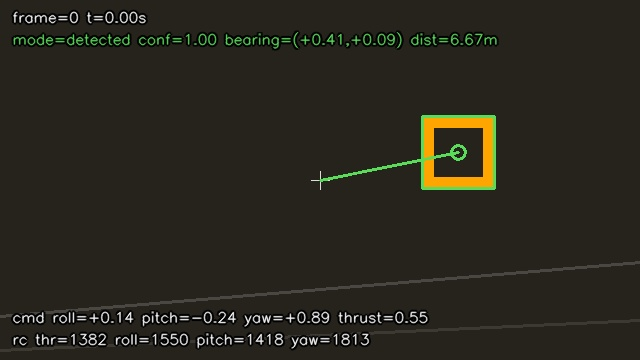
\includegraphics[width=\columnwidth]{gate_sequence_detected.jpg}
\caption{Example FPV gate detection used by the current classical perception stack. The detector provides bearing, confidence, and approximate range rather than a dense scene representation.}
\label{fig:gate-detection}
\end{figure}

The reactive controller converts these detector outputs into flight commands. Horizontally, image bearing error drives yaw and lateral roll commands. Vertically, image elevation and the known 20 degree camera tilt drive pitch and thrust. Distance controls forward aggressiveness and commit behavior. In search mode, the controller should settle and hover before yawing, because yawing while pitched forward causes an off-axis spiral.

This controller is useful as a baseline and as a data-quality diagnostic, but it is not robust enough for aggressive racing. It only reacts to the current apparent gate center. It does not know the gate normal, future curvature, or how the next gate should enter the camera after passing the current one. That is why the learning pipeline uses a privileged teacher for labels.

\section{Privileged Teacher and Student Policy}

The teacher is privileged only during data generation. It can use the debug course geometry: ordered gate centers, gate yaw, and therefore gate normals. It generates a smooth racing line and selects a lookahead point along that line. Commands are then produced from the vehicle state to rejoin or follow the line. The deployed policy never receives the true gate center, gate ID, global pose, or simulator gate normal.

This separation is important. It allows high-quality labels while preserving the competition input constraint:

\begin{center}
\small
\begin{tabular}{ll}
\toprule
Teacher input & Student input \\
\midrule
Gate centers and normals & Detected gate bearing \\
Course order & Tracker mode and confidence \\
World pose for scoring & Approximate range and image size \\
Racing-line lookahead & Telemetry and short history \\
\bottomrule
\end{tabular}
\end{center}

The first learned controller is a GRU/MLP policy. At each timestep, it receives detector/tracker features and telemetry. The GRU keeps temporal memory through brief detector drops, fast turns, and partial occlusions. A small MLP head outputs the same body-rate/thrust command as the reactive controller. This is a behavior-cloning stage, not reinforcement learning.

\section{Course Curriculum}

Simple straight tracks are not enough to evaluate the algorithm. They can make a controller look competent even if it only points at the nearest visible gate. I therefore added harder curved courses: circular arcs, S-curves, randomized S-curves, randomized arcs, and hard S-curves with stronger lateral displacement. Figure~\ref{fig:racing-lines} shows the privileged teacher racing lines and gate normals.

\begin{figure*}[t]
\centering

\includegraphics[width=\textwidth]{teacher_racing_lines_curve_stress_full.png}
\caption{Privileged teacher racing lines for base, randomized, and held-out curved courses. Gate arrows visualize pass direction from gate yaw, which is the teacher-side gate normal information that should eventually be estimated by perception.}
\label{fig:racing-lines}
\end{figure*}

The current camera model is mostly adequate for the next gate, but lookahead becomes weak on hard curves. In the VQ1 pinhole profile, the held-out hard S-curve keeps the next gate visible 99.3\% of the time, but the lookahead point visible only 80.9\% of the time. A wider experimental fisheye profile improves hard-curve lookahead visibility to 99.9\%, but it is not the default competition profile. This motivates learning a policy that can use temporal memory and gate geometry, not just instantaneous center tracking.

\begin{table}[t]
\centering
\small
\begin{tabular}{lccc}
\toprule
Profile & Course & Next visible & Lookahead visible \\
\midrule
VQ1 pinhole & hard S & 99.3\% & 80.9\% \\
Wide fisheye & hard S & 99.9\% & 99.9\% \\
VQ1 pinhole & S-curve & 100.0\% & 99.8\% \\
\bottomrule
\end{tabular}
\caption{Visibility audit for curved tracks. The pinhole camera is enough for ordinary S-curves, but hard curve lookahead can leave the field of view.}
\label{tab:fov}
\end{table}

\section{Experiments}

The experiments evaluate three levels of progress.

\paragraph{Reactive baseline.}
On the easier practice courses, the visual-servo controller completes straight and mild-offset layouts. On harder curved courses, it fails: circular arc reaches 2/4 gates and S-curve reaches 1/5 gates within the 16 second run. This is useful because it reveals that the project needs sequence-aware navigation rather than just better color detection.

\paragraph{Offline imitation.}
The curve-stress teacher dataset contains 34 courses and 25,812 labeled rows after adding corridor recovery examples. It includes nominal racing-line states, launch states, off-nominal recovery states, and first-gate corridor states. The best corridor-policy checkpoint reached validation MSE 0.00283 and held-out hard-S-curve MSE 0.00483. On the same trace, the learned policy matched the teacher much better than the reactive controller: learned-vs-teacher MSE was 0.00474, while reactive-vs-teacher MSE was 0.21254.

\begin{table}[t]
\centering
\small
\begin{tabular}{lc}
\toprule
Metric & Value \\
\midrule
Teacher rows & 25,812 \\
Courses & 34 \\
Best validation MSE & 0.00283 \\
Held-out hard S MSE & 0.00483 \\
Learned vs. teacher MSE & 0.00474 \\
Reactive vs. teacher MSE & 0.21254 \\
\bottomrule
\end{tabular}
\caption{Offline behavior cloning result for the corridor curriculum. Offline fit improved substantially, but it is not sufficient evidence of closed-loop success.}
\label{tab:offline}
\end{table}

\paragraph{Closed-loop validation.}
Closed-loop validation was less successful. A short S-curve run with the corridor checkpoint still failed to pass gate 0. The lateral miss improved compared with the previous DAgger checkpoint: at about 7 seconds, the previous checkpoint was at $y=-4.77$ m, while the corridor checkpoint was at $y=-2.53$ m. However, the run still did not complete the first gate. A later trace audit also showed that the safety supervisor kept the system in \texttt{reactive\_fallback} for much of the run, meaning the learned policy was not actually receiving full authority. This is a critical finding: PPO should not begin until closed-loop command authority and adapter scaling are verified.

\section{Discussion}

The main lesson is that offline imitation loss can be misleading in drone racing. A policy can match teacher commands on logged states but fail once its own small errors change the future state distribution. This is exactly the setting where DAgger is useful: run the student closed-loop, collect the states where it drifts, relabel those states with the privileged teacher, and retrain.

The second lesson is that the detector output is currently too weak for high-speed curved racing. A neural gate detector would ideally provide not only a center point, but also corners, range, gate plane orientation, and uncertainty. From a single calibrated image, known gate geometry can estimate a relative pose through PnP. That relative pose can give the student features closer to what the privileged teacher uses: lateral offset, range, yaw-to-gate-normal, and a pass-through direction. This would make the GRU policy more like a learned navigation controller and less like a smoothed image-center servo.

The third lesson is that the output adapter matters. The same learned body-rate command can behave differently after Betaflight RC scaling or MAVSDK attitude-rate conversion. The next engineering test is an adapter-scale sweep and command-source audit: the trace must show when commands come from the learned policy versus fallback, and the vehicle response must be compared against the commanded lateral/yaw correction.

\section{Next Steps}

The planned roadmap is:

\begin{enumerate}
  \item Keep the classical detector as the feature extractor until it clearly bottlenecks the system.
  \item Add richer gate features: corner geometry, range, estimated gate normal, and uncertainty.
  \item Run DAgger with learned-only relabeling on closed-loop drift states.
  \item Validate on circular arcs, S-curves, and held-out hard S-curves.
  \item Only then use PPO or another RL method for fine-tuning.
\end{enumerate}

For PPO, the action space can remain body rates and thrust. The observation should initially remain feature-based rather than raw pixels. This is the most realistic use of a single T4 GPU and limited cloud budget. Raw-image RL or world-model training would be much more expensive and harder to debug.

\section{Conclusion}

This project reset the autonomous drone racing system around the correct competition boundary: FPV and telemetry in, body-rate/thrust commands out. The current reactive controller proves the perception and command pipeline on simple tracks, but curved tracks reveal the need for learned temporal control and better gate geometry. The privileged teacher pipeline provides a practical path forward: use privileged simulator geometry only to generate labels, train a legal feature-policy student, then close the loop with DAgger before attempting PPO. The immediate research direction is not just ``train a bigger model,'' but give the policy the right gate features and validate that its commands actually control the drone in closed loop.

\begin{thebibliography}{9}

\bibitem[Kaufmann et~al.(2023)]{kaufmann2023champion}
Elia Kaufmann, Leonard Bauersfeld, Antonio Loquercio, Matthias Mueller, Vladlen Koltun, and Davide Scaramuzza.
\newblock 2023.
\newblock Champion-level drone racing using deep reinforcement learning.
\newblock \emph{Nature}.

\bibitem[Loquercio et~al.(2021)]{loquercio2021learning}
Antonio Loquercio, Elia Kaufmann, Rene Ranftl, Matthias Mueller, Vladlen Koltun, and Davide Scaramuzza.
\newblock 2021.
\newblock Learning high-speed flight in the wild.
\newblock \emph{Science Robotics}.

\bibitem[Mellinger and Kumar(2011)]{mellinger2011minimum}
Daniel Mellinger and Vijay Kumar.
\newblock 2011.
\newblock Minimum snap trajectory generation and control for quadrotors.
\newblock In \emph{IEEE International Conference on Robotics and Automation}.

\bibitem[Ross et~al.(2011)]{ross2011dagger}
Stephane Ross, Geoffrey Gordon, and Drew Bagnell.
\newblock 2011.
\newblock A reduction of imitation learning and structured prediction to no-regret online learning.
\newblock In \emph{AISTATS}.

\bibitem[Schulman et~al.(2017)]{schulman2017ppo}
John Schulman, Filip Wolski, Prafulla Dhariwal, Alec Radford, and Oleg Klimov.
\newblock 2017.
\newblock Proximal policy optimization algorithms.
\newblock \emph{arXiv preprint arXiv:1707.06347}.

\end{thebibliography}

\end{document}
